\subsection{Free Energy}
\begin{frame}{Free Energy Calculations}
\begin{itemize}
	\item Solvent-solvent interactions heavily dominate Dynamics energies
	\vspace{1 cm}
	\item Impossible to directly extract binding energies
	\vspace{1 cm}
	\item Use thermodynamics cycles to approximate relative energies
\end{itemize}
\end{frame}

\begin{frame}{Free Energy Methods (GBSA)}
\begin{columns}
\column{0.5\textwidth}
\begin{itemize}
		\item Postprocessing technique to approximate free energy
		\vspace{1 cm}
		\item Uses implicit solvent
		\vspace{1 cm}
		\item Estimates entropy
\end{itemize}
\column{0.5\textwidth}
\begin{figure}
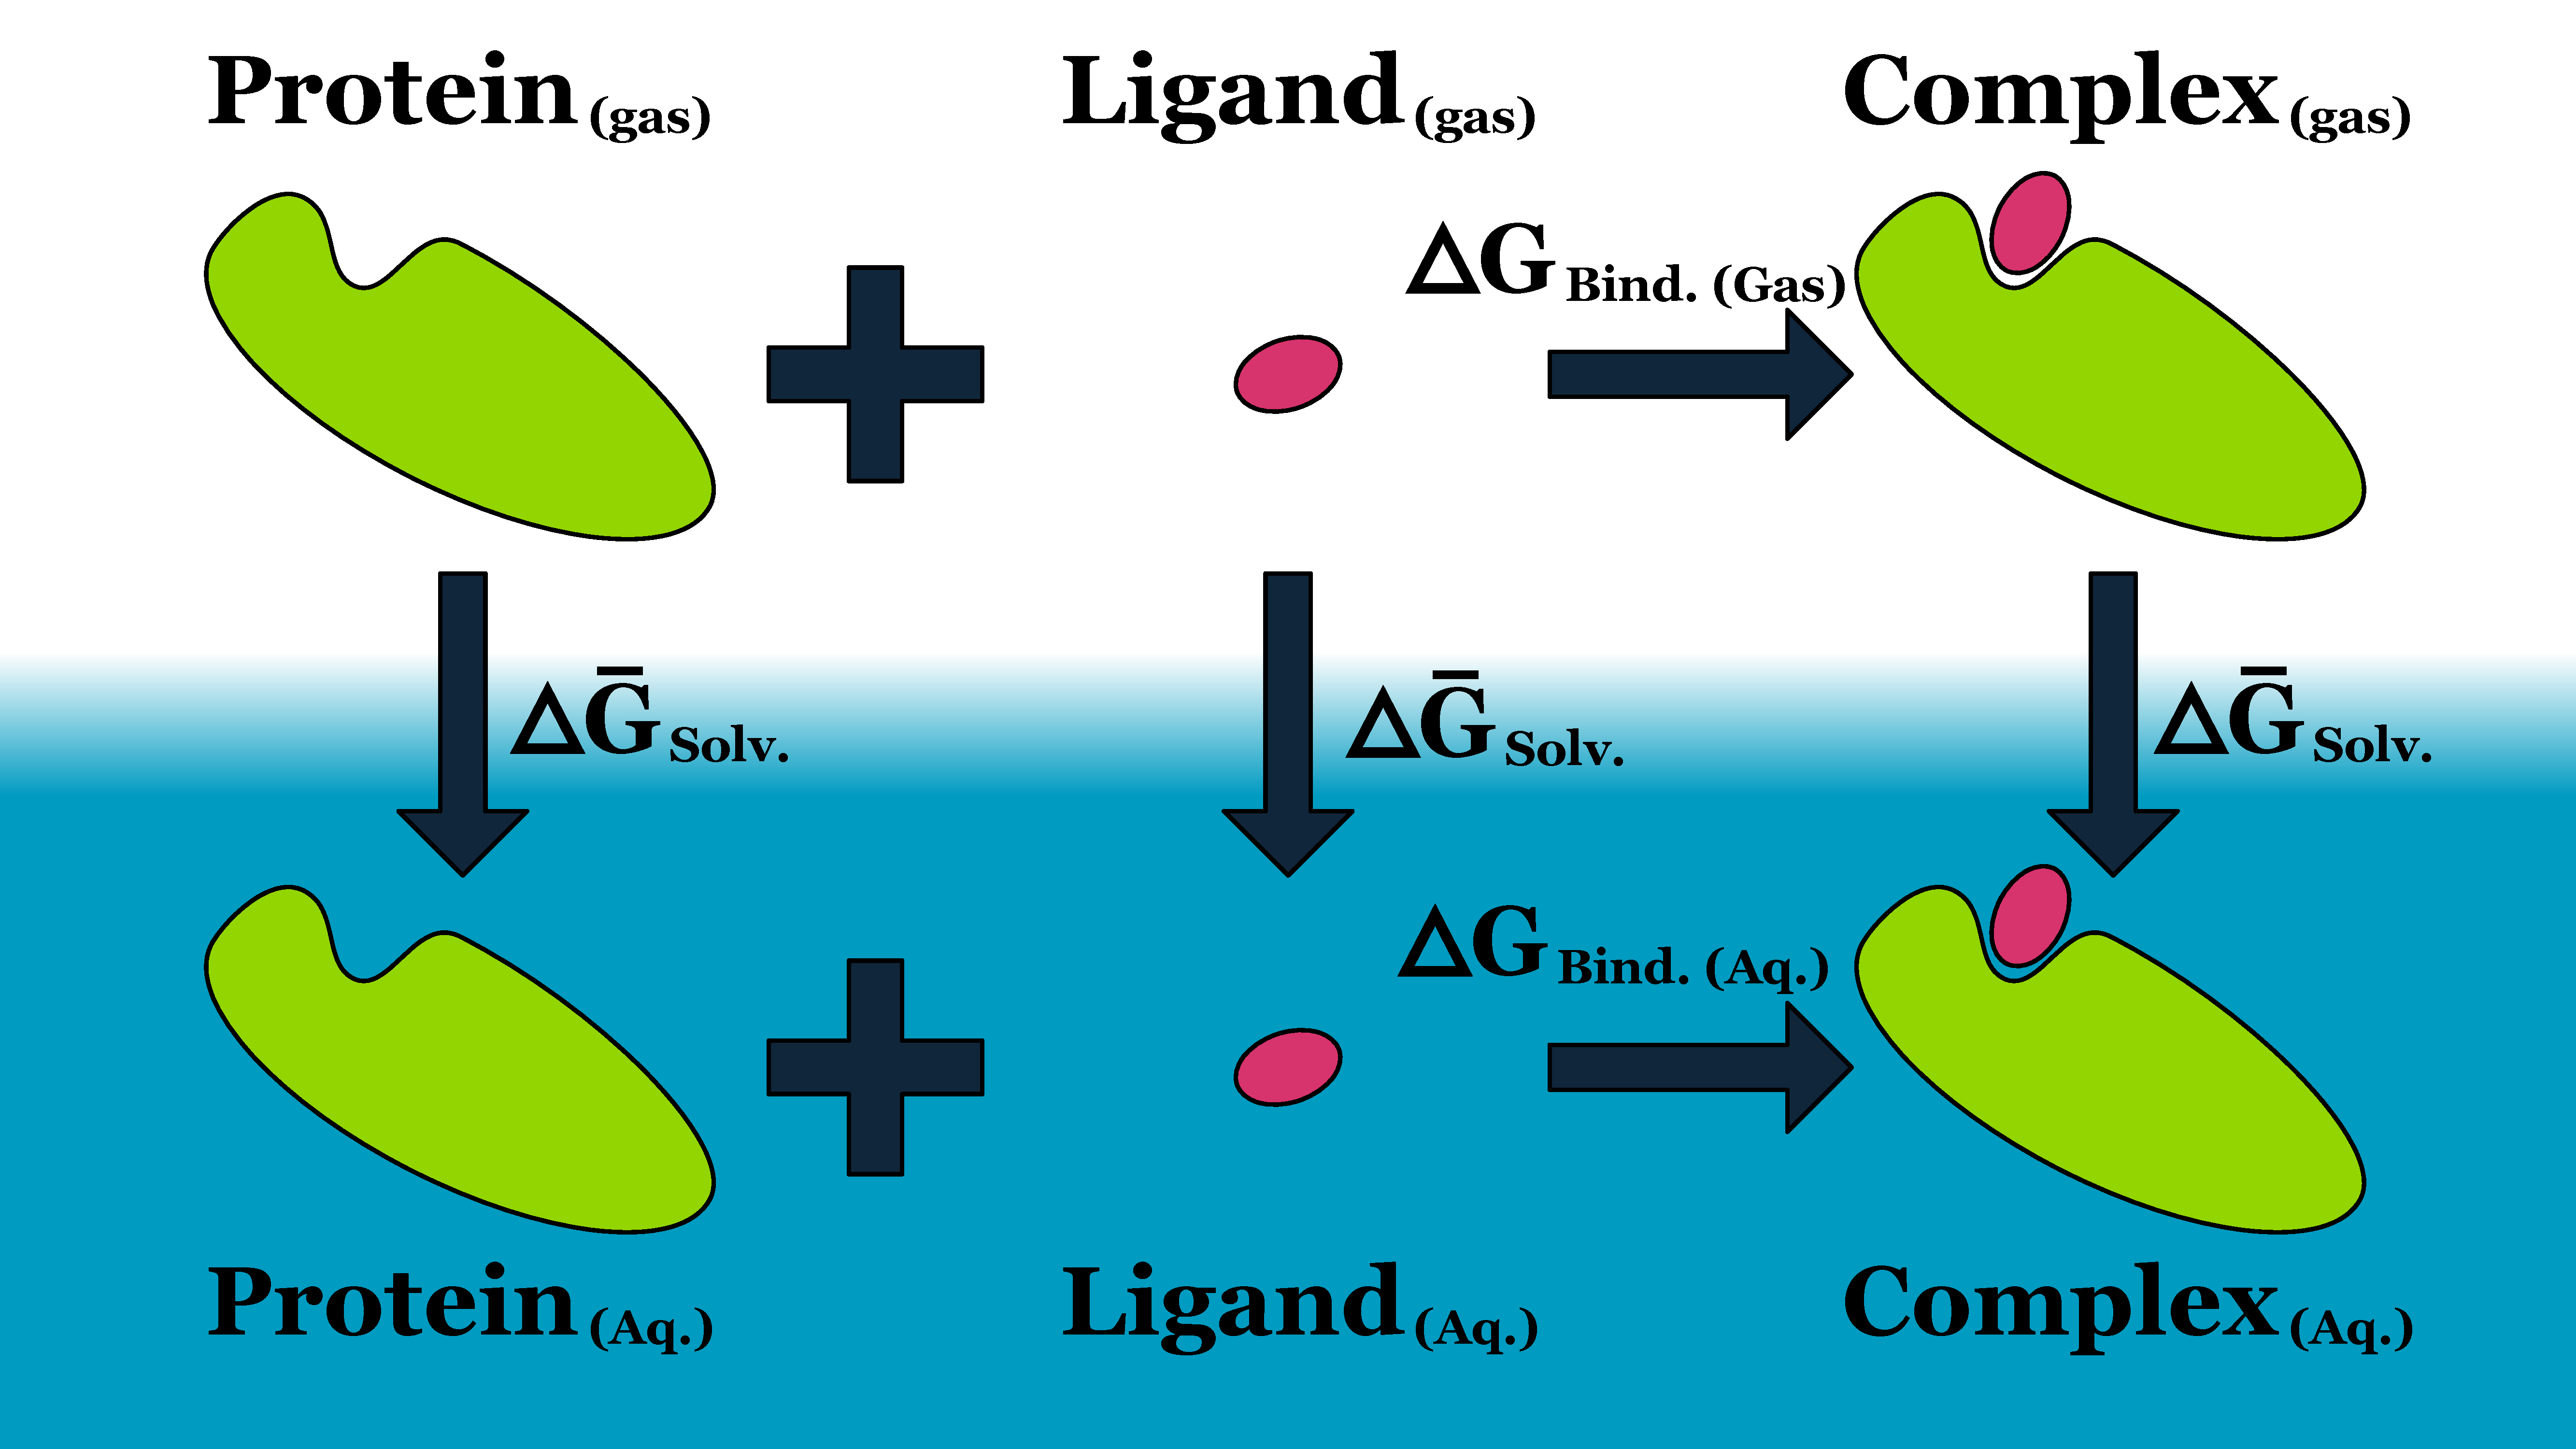
\includegraphics[width=0.95\textwidth]{../Graphics/Theory/gbsa}
\end{figure}
\begin{equation}
        \Delta G_{bind} = \Delta \bar{G}_{complex} - \Delta \bar{G}_{prot.} - \Delta \bar{G}_{lig.}
\end{equation}
\end{columns}
\end{frame}

\begin{frame}{Free Energy Methods (Higher Level)}
\begin{columns}
\column{0.5\textwidth}
\begin{itemize}
	\item Umbrella Sampling
	\vspace{0.8 cm}
	\item Free Energy Perturbation
	\vspace{0.8 cm}
	\item QMMM hybrid methods
	\vspace{0.8 cm}
	\item Thermodynamic Integration
\end{itemize}
\column{0.5\textwidth}
\begin{figure}
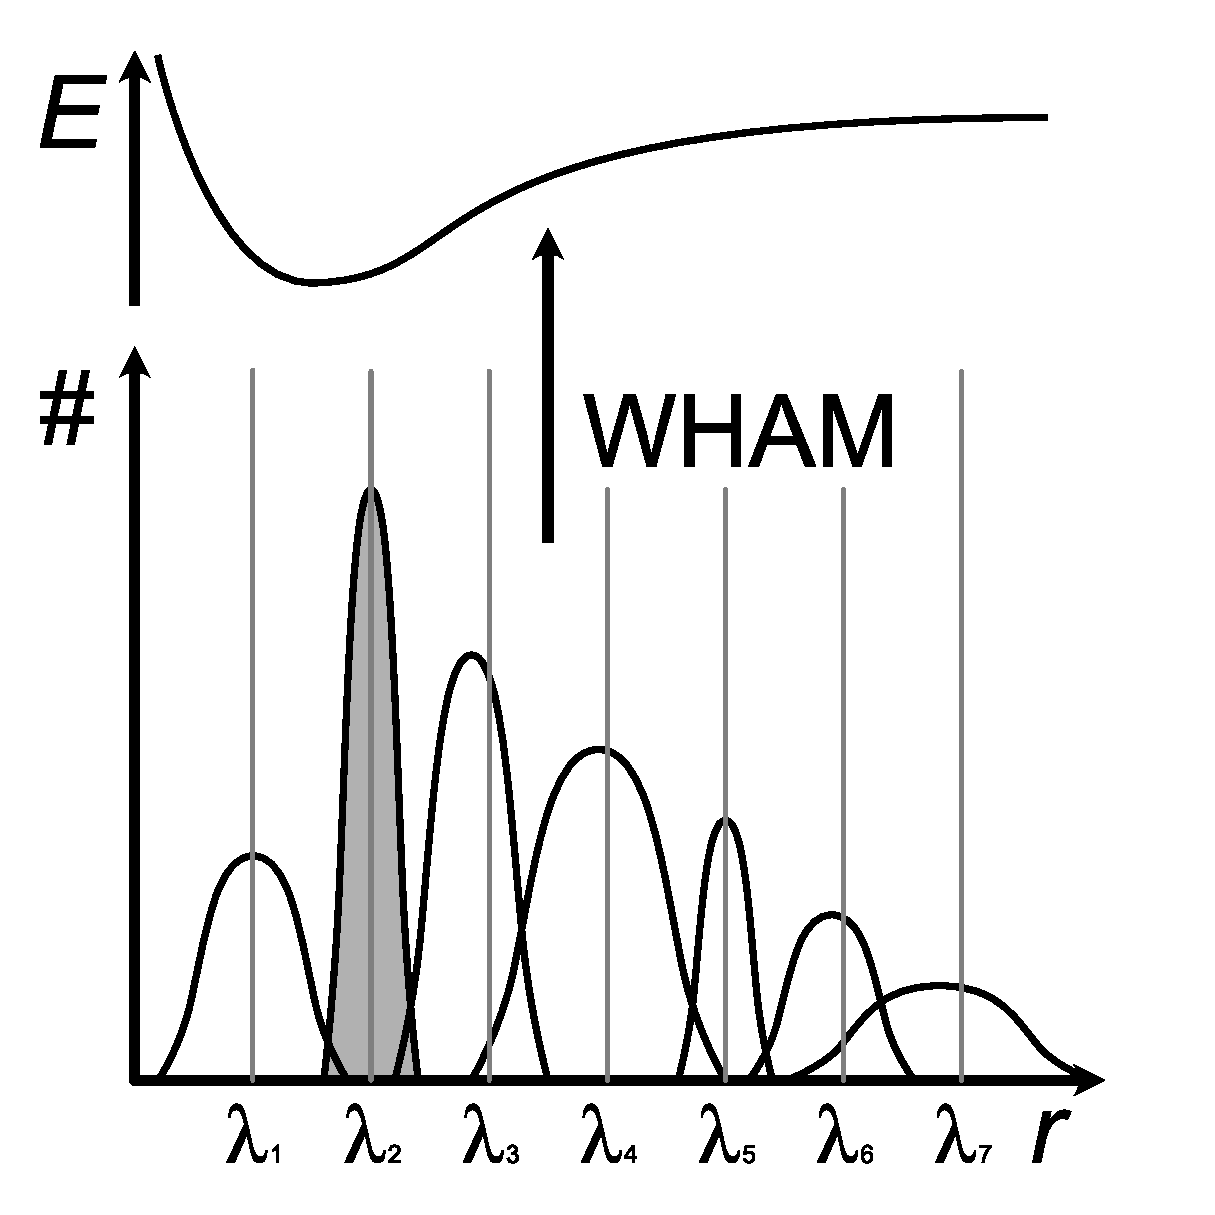
\includegraphics[height=0.35\textheight]{figures/Me/Wham_Hist}
\end{figure}
\begin{figure}
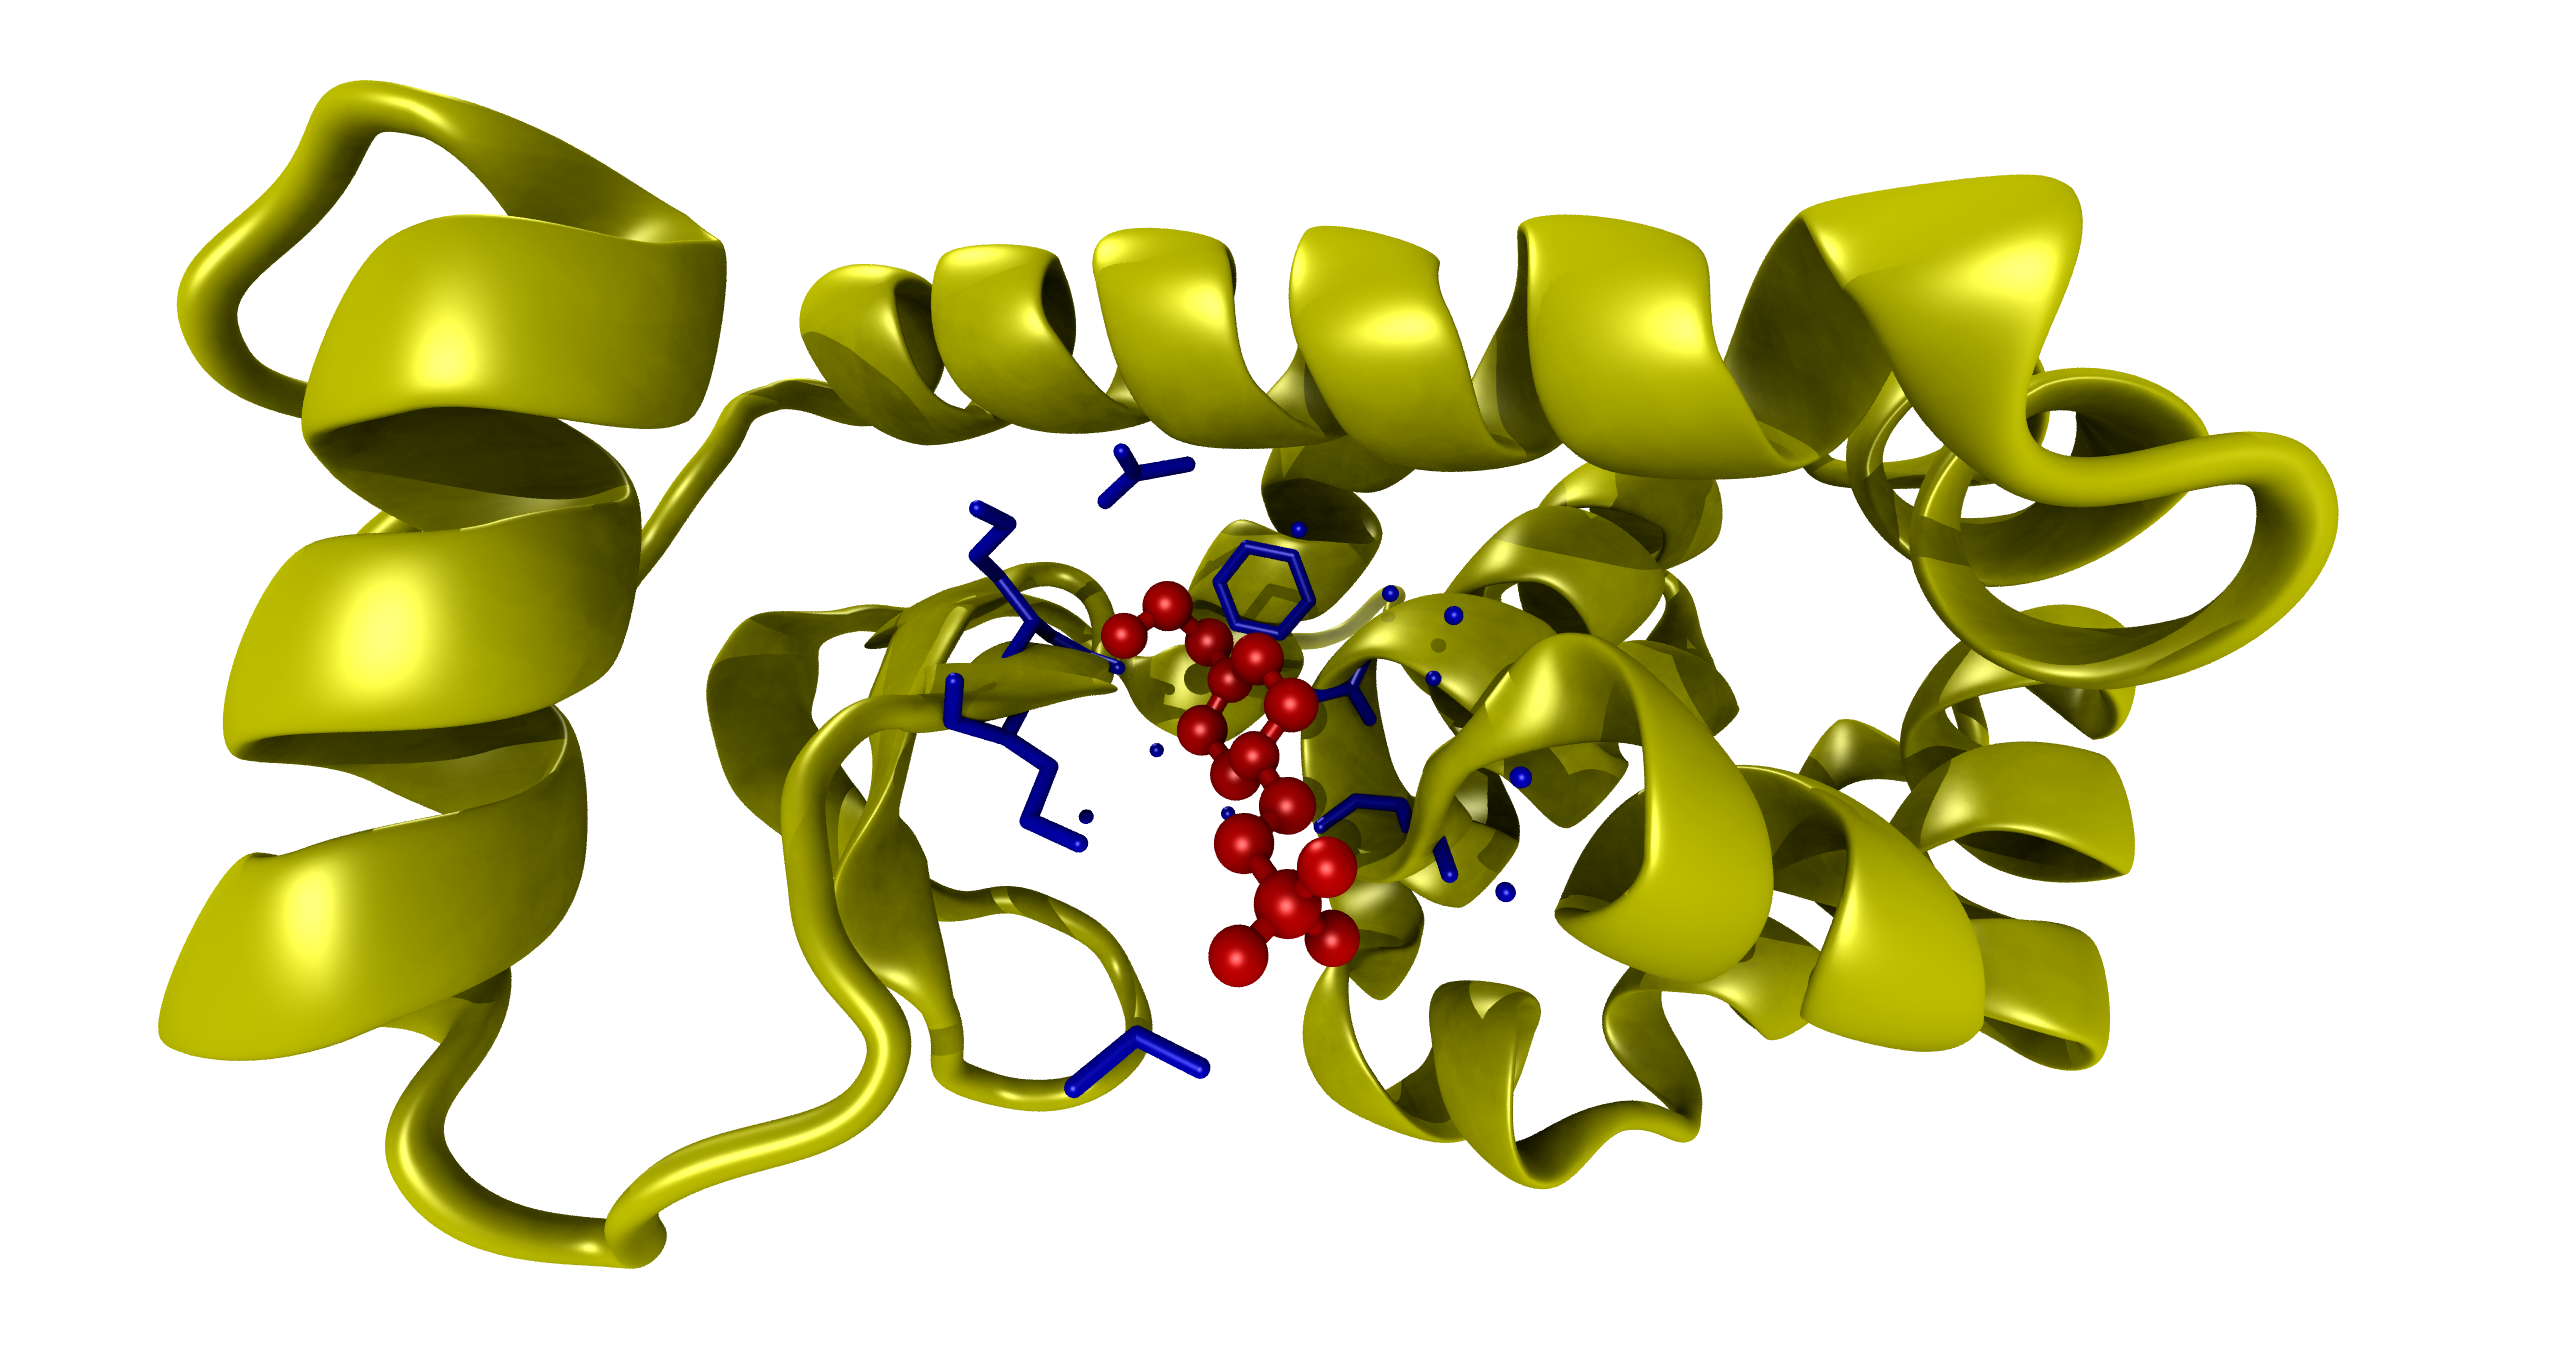
\includegraphics[height=0.35\textheight]{../Graphics/Theory/QMMM.png}
\end{figure}
\end{columns}

\end{frame}